\begin{python}
    # Slider
    self.dashboard <= w.label('Slider', typo='headline4', style=flex)
    self.dashboard <= w.slider(
        'Slider',
        min=1,
        max=10,
        step=0.1,
        value=5,
        on_change=self.on_slider,
        id='my_slider',
    )
    self.dashboard <= w.label(
        f'', id='for_slider', typo=f'body1', style=flex
    )

    # Slider range
    self.dashboard <= w.label('Slider range', typo='headline4', style=flex)
    self.dashboard <= w.range_slider(
        'Slider range',
        min=0,
        max=20,
        value_lower=5,
        value_upper=15,
        step=1,
        on_change=self.on_slider_range,
        id='my_range',
    )
    self.dashboard <= w.label(f'', id='for_range', typo=f'body1', style=flex)


def on_slider(self, value):
    # value = w.get_value('my_slider')
    document.select_one('#for_slider').html = f'Slider Changed: {value}'


def on_slider_range(self, value):
    # value = w.get_value('my_slider')
    document.select_one('#for_range').html = f'Range Changed: {value}'
\end{python}


\begin{figure}[H]
\begin{centering}
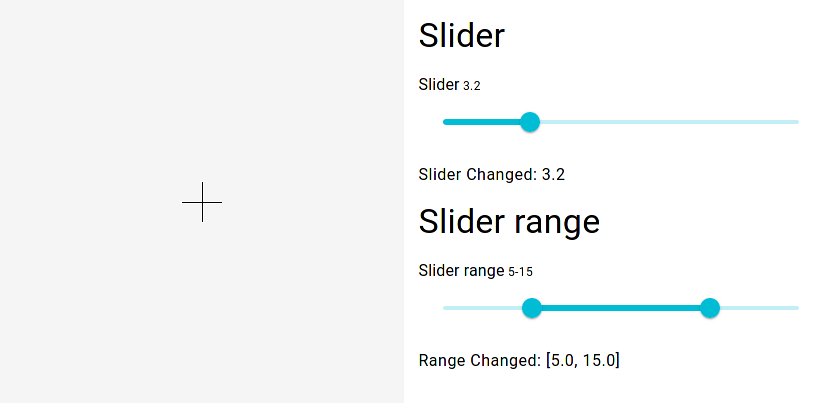
\includegraphics[scale=0.5]{Cap4/Figures/widgets/sliders.png}
\par\end{centering}
\caption[Brython Radiant: Slider]{Brython Radiant: Sliders.}
\label{fig:radiant_sliders}
\end{figure}